%\svnkwsave{$RepoFile: siminos/blog/energy.tex $}
%\svnidlong {$HeadURL: svn://zero.physics.gatech.edu/siminos/blog/energy.tex $}
%{$LastChangedDate: 2017-03-12 23:45:05 -0400 (Sun, 12 Mar 2017) $}
%{$LastChangedRevision: 4627 $} {$LastChangedBy: predrag $}
%\svnid{$Id: energy.tex 4627 2016-02-07 01:48:53Z predrag $}

\chapter{Energy, dissipation, invariant moments}
\label{c-energy}

\renewcommand{\ssp}{x}             % state space point

\begin{description}
\item[2008-06-26 PC] moved this to Siminos thesis from
        \texttt{blog/flotsam.tex}.
\item[2009-10-02 PC] moved this back again from
        \texttt{blog/flotsam.tex}.
\item[2012-03-27 PC] In rev.~2294 moved this to
        \texttt{siminos/baroclinic/PCnotes.tex}.
\item[2012-06-06 ES]
Text on invariant moments resurrected from rev. 903. Apparently
disappeared in rev. 904, committed by Predrag. I don't know whether this
excerpt was moved elsewhere. Also I did not try to check whether some
other useful excerpt went MIA in that commit.

\item[2012-06-06 PC] Thanks for amazing detective work! The most
up-to-date version is currently in
\texttt{siminos/baroclinic/PCnotes.tex}, there to persuade Annalisa
and Sebastian to plot some \statesp\ invariants cheaply.

\item[2013-03-31 PC] Annalisa and Sebastian showed no interest, so
the text is back as \texttt{siminos/blog/energy.tex}.

Also search for {\bf 2011-12-06, 2012-02-14 PC} in
\texttt{siminos/lyapunov/blog.tex}.

\item[2013-04-04 PC] Moved exercises and text edits to
ChaosBook.org chapter PDEs.tex

\end{description}

\section{\KSe}
\label{s-KS}

The \KS\ system\rf{KurTsu75,siv} is given by
\beq
  u_t = F(u) = -{\textstyle\frac{1}{2}}(u^2)_x-u_{xx}-u_{xxxx}
    \,,\qquad   x \in [-L/2,L/2]
    \,.
\ee{ks}

\subsection{Energy transfer rates for $L=22$ case}
\label{sec:energyL22}

%%%%%%%%%%%%%%%%%%%%%%%%%%%%%%%%%%%%%%%%%%%%%%%%%%%%%%%%%%%%%%%%
\begin{figure}[t]
\begin{center}
 \begin{tabular}{cc}
        ~~~~~~~~(\textit{a})                        &   ~~~~~~~~(\textit{b}) \\
    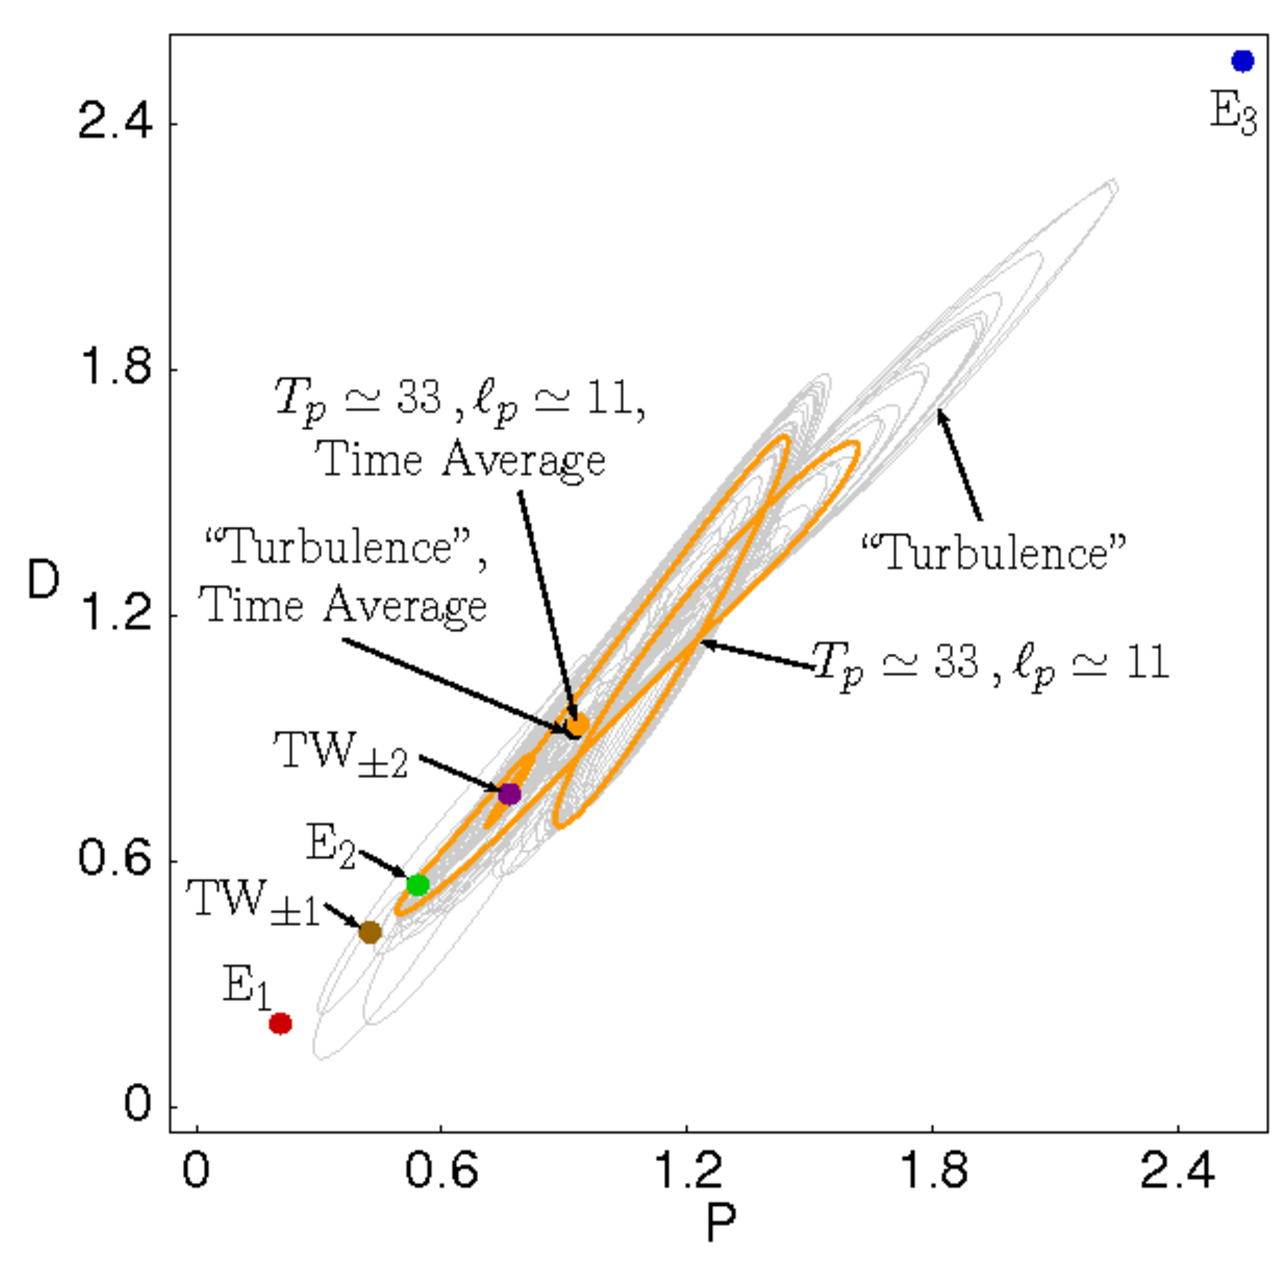
\includegraphics[width=0.46\textwidth, clip=true]{energyBalance_pst}
    & 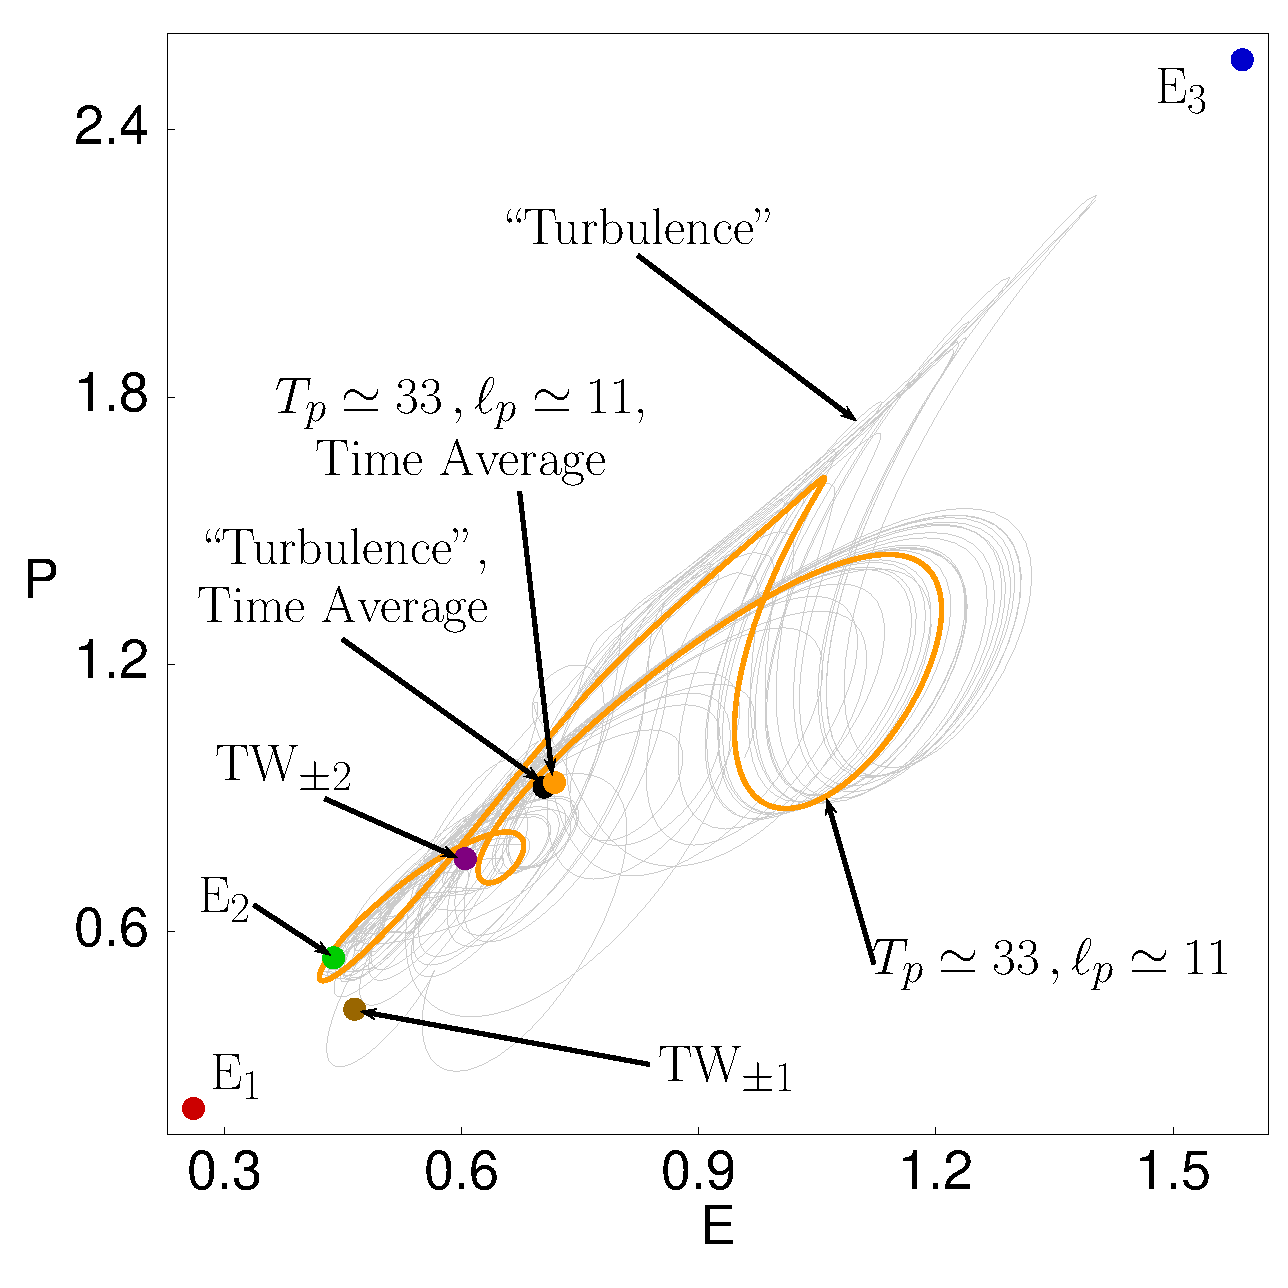
\includegraphics[width=0.46\textwidth, clip=true]{equivaEP_pst}

  \end{tabular}
\end{center}
\caption{
(a) Power input $P$ {\em vs.}
dissipation rate $D$
(b) energy $E$  {\em vs.}
power input $P$,   for several  \eqva\ and \reqva,
a \rpo, and a typical `turbulent' long-time trajectory.
System size $L=22$.
        }
\label{f:drivedrag1}
\end{figure}
%%%%%%%%%%%%%%%%%%%%%%%%%%%%%%%%%%%%%%%%%%%%%%%%%%%%%%%%%%%%%%%%%%

%%%%%%%%%%%%%%%%%%%%%%%%%%%%%%%%%%%%%%%%%%%%%%%%%%%%%%%%%%%%%%%%
\begin{figure}[t]
\begin{center}
 \begin{tabular}{cc}
        ~~~~~~~~(\textit{a})                        &   ~~~~~~~~(\textit{b}) \\
    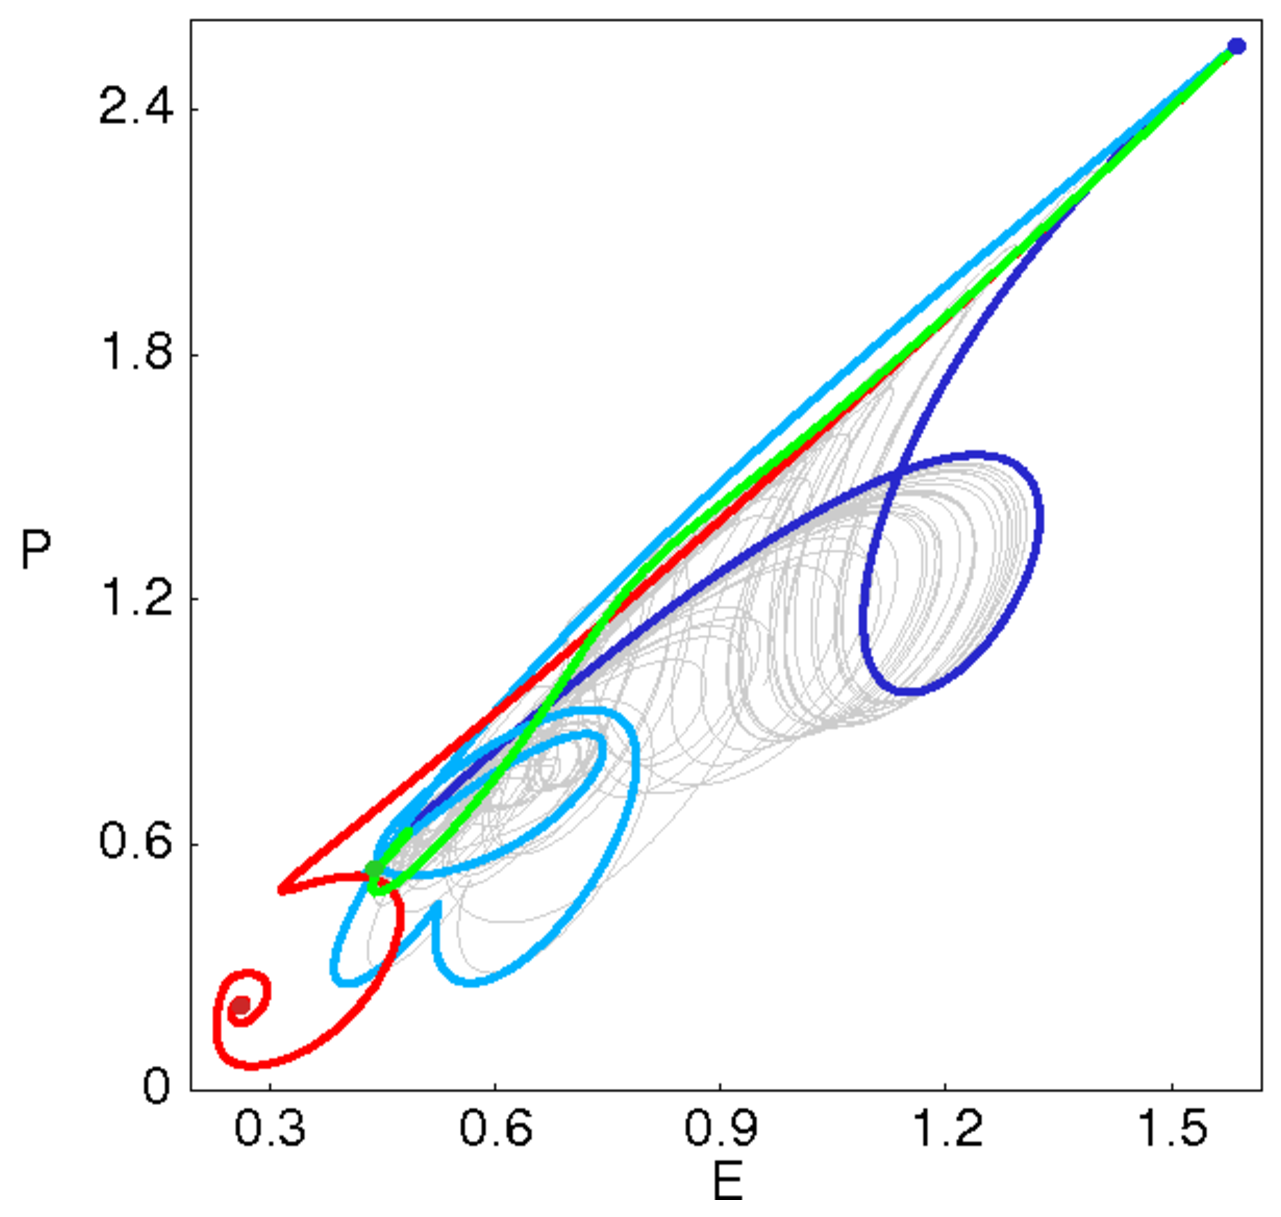
\includegraphics[width=0.46\textwidth, clip=true]{connEP}
     & 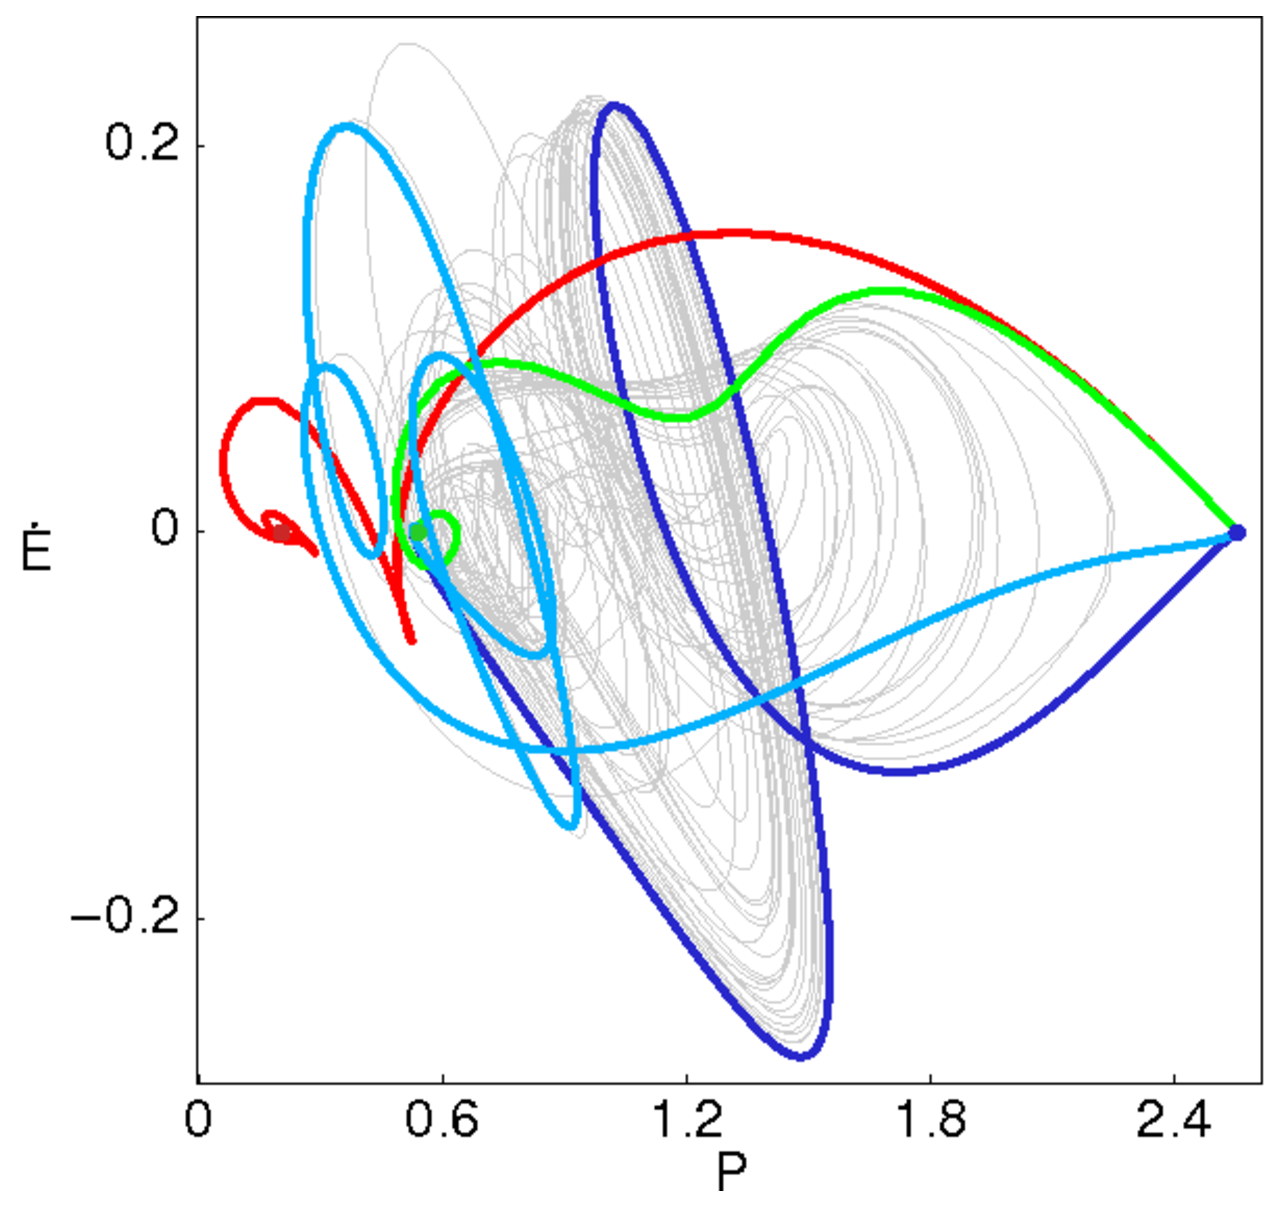
\includegraphics[width=0.46\textwidth, clip=true]{connPEdot}
 \end{tabular}
\end{center}
\caption{
Two projections of the $(E,P,\dot{E})$ representation of the flow.
\EQV{1} (red), \EQV{2} (green), \EQV{3} (blue),
\hec s from \EQV{2} to $\EQV{3}$ (green),
from $\EQV{1}$ to \EQV{3} (red)
and from \EQV{3} to $\EQV{2}$ (shades of blue), superimposed over
a generic long-time `turbulent' trajectory (grey).
System size $L=22$.
        }
\label{f:drivedragConn}
\end{figure}
%%%%%%%%%%%%%%%%%%%%%%%%%%%%%%%%%%%%%%%%%%%%%%%%%%%%%%%%%%%%%%%%%%

                                                    \toCB
In \reffig{f:drivedrag1} we plot %\refeq{EnRate},
the time-dependent
$\dot{\expctE}$ in the power input $P$ {\em vs.}
dissipation rate $D$ plane, for $L=22$ \eqva\ and \reqva,
a selected \rpo, and for a typical `turbulent' long-time
trajectory.

Projections from the $\infty$-dimensional \statesp\ onto the 3-dimensional
$(E,P,D)$ representation of the flow, such as
\reffigs{f:drivedrag1}{f:drivedragConn}, can be misleading.
The most one can say is that if points are clearly separated in an
$(E,P,D)$ plot (for example, in \reffig{f:drivedrag1}
$\EQV{1}$ \eqv\ is outside the recurrent set), they are also separated
in the full \statesp.  Converse is not true -- states of
very different topology can have similar energies.

An example is the \rpo\ \RPO{2} $(\period{p},\shift_p) = (32.8,10.96)$
which {is the least unstable short \rpo\ we have detected in this system.
It} appears to be well embedded within the turbulent flow. The mean power
$\timeAver{P_p}$,
% evaluated as in \refeq{poE},
see \reffig{f:drivedrag1},
is numerically quite close to the long-time turbulent time average
$\timeAver{P}$.

\subsection{Further observables, \KS}
\label{sec:moreObs}

                                                    \toCB
This section contains some material which has not been included in
publications and/or Siminos and Lan Ph.D. theses.

{\bf PC}: believe it or not, we are now set to compute
    $\timeAver{E}$ and $\timeAver{P}$
    using cycle expansions

Substitution % by \refeq{KSeqvCond}
verifies that for an \eqv\ $\expctE$ is constant:
\[
   \dot{\expctE} =
\expct{ \left({u^2}/{2} + u_{x} + u_{xxx} \right) u_x}
    = \expctE \expct{ u_x }=0
    \,.
\]


% PC worked out in part with Bridges
An infinite number of identities for moments of
solutions of KS follow\rf{Bridges_priv}. For example,
integrating by parts $\expct{u_{x} u_t}$,
$\expct{u_{xx} u_t}$,
and
$\expct{u^2 u_t}$,
respectively, one obtains \reqva\ relations
\PC{please re-derive these three. Are there more
    important ones that I have missed?
    Also, I - unnecessarily - specialized to \reqva,
    but these identities will be especially useful for \rpo s}
\RLD{I don't quite follow this process of deriving moments.  What is
the reason we look for some combinations of $u$ and its derivatives?
Why not just take $\expct{u_{x\cdots x}}$?
Is there any physical motivation for such combinations,
beyond $E$, $P$ and $D$?  Maybe use things like $\dot{P}$,
$\dot{D}$, etc.?}
\PC{they merit more thought and time than we have now, so let's
   pick them up after the first paper is submitted}
\bea
% \expct{u_{x} u_t}
%     \qquad \to \qquad
c P &=& \expct{u \, u_{x}{}^2}
\label{Bridges1}\\
c P  &=& \expct{u \, u_{xx}{}^2}
\label{Bridges3}
\,.
\eea
True for any solution:
\bea
% \expct{u_{xx} u_t}
%     \qquad \to \qquad
\dot{P} &=& 2P - \expct{u_{x}{}^3}  - 2 \expct{u_{xxx}{}^2}
\label{PC1}\\
\dot{D} &=& 2\expct{u_{xxxx}{}^2}
    + 5 \expct{u_{xx}{}^2 u_{x}}  - 2 \expct{u_{xxx}{}^2}
\label{PC2} \\
\ddot{E} &=& \dot{P} - \dot{D} =
     2P - \expct{u_{x}{}^3}
    - 2\expct{u_{xxxx}{}^2} - 5 \expct{u_{xx}{}^2 u_{x}}
\label{PC4}\\
\frac{d}{dt} \expct{u_{x}{}^3} &=&
        3 \expct{u_{x}{}^3u + u_{xx}{}^3}
\label{PC5}
\,.
\eea
When moments such as \refeq{Bridges1} are added as
coordinate axes to \reffig{f:drivedragConn}, \reqva\ and
\rpo s are separated from \eqva\ and \po s. Furthermore,
as higher moments have more and more powers of $u$ and derivatives
$u_{xx\cdots x}$, their magnitudes should be strongly suppressed,
providing a symmetry-invariant basis set that can be safely truncated to
a finite-dimensional \statesp.

For example, the energy of \reqva\ \REQV{\pm}{2} which
seems close to the
mean turbulent energy in \reffig{f:drivedrag1} is separated
from it when plotted along the
$\expct{u \, u_{x}{}^2}$ moment, where according to
\refeq{Bridges1} it takes nonzero value $c P$.

%%%%%%%%%%%%%%%%%%%%%%%%%%%%%%%%%%%%%%%%%%%%%%%%%%%%%%%%%%%%%%%%%%%%%%%%%%
% \ifboyscout\else\newpage\fi

\exercise{Channelflow.org.}{ \label{exer:channelflow}
% Predrag                           1apr2013
(Bonus) Please download the code.
\HREF{http://channelflow.org/dokuwiki/doku.php?id=docs:tutorial}{Tutorial}
and
\HREF{http://channelflow.org/dokuwiki/doku.php?id=gtspring2009:howto}
{HowTo}
might be helpful.
        }% end \exercise{\KS\ energy transfer rates




    \renewcommand{\inputfile}{\version\ - edited 2008-06-26 bronski-2005}
\section*{Uncertainty estimates and $L_2$ bounds for the Kuramoto-Sivashinsky equation}
% $Author: predrag $ $Date: 2008-06-26 10:30:57 -0400 (Thu, 26 Jun 2008) $

Jared C. Bronski
%\footnote{Department of Mathematics,
% University of Illinois Urbana-Champaign, 1409 W. Green St, Urbana IL 61801}\\
and
Tom Gambill

importance as a model for flame fronts\cite{siv} and
phase turbulence\cite{KS}
and plasmas\cite{LMRT} the
KS equation has become
one of the canonical models for
spatio-temporal chaos in $1\!+\!1$ dimensions
\cite{JOHNSON,KEVREKIDIS,Man}.

Nicolaenko, Scheurer and Temam\cite{NICO} gave the first long-time
boundedness result for the Kuramoto-Sivashinsky equation, showing
 that $\limsup_{t \rightarrow \infty} |\!|u|\!|_2
\le C L^{\frac{5}{2}}$
for odd initial data, as well as showing
that bounds on the $L_2$ norm imply bounds on the dimension of the attractor.

The $L_2$ estimate was improved by
Collet, Eckmann, Epstein and
Stubbe\cite{CEES} who  extended it to any mean-zero initial data and improved the exponent from
$\frac{5}{2}$ to $\frac{8}{5}$,
and by Goodman\cite{Good}, who extended it to
any mean-zero initial data with the same exponent.

these papers that the function $|\!|u-\phi|\!|_2^2$ is a Lyapunov function for
an appropriately chosen $\phi$ and $|\!|u|\!|_2$ sufficiently large.

bounds which do not fit into Lyapunov function framework:
Ilyashenko\cite{Ilyashenko},
Otto  and Giacomelli\cite{GO}.
The latter, which treats the KS equation as a
perturbation of the Burger's equation, is currently the best estimate, establishing that
\[
\limsup_{t \rightarrow \infty} |\!|u|\!|_2 = o(L^{\frac{3}{2}}).
\]

In this paper we give an elementary argument of the Lyapunov function
type which establishes the slightly weaker result
\[
\limsup_{t \rightarrow \infty} |\!|u|\!|_2 = O(L^{\frac{3}{2}}).
\]
Our proof applies equally to the destabilized Kuramoto-Sivashinsky (dKS)
equation:
\[
u_t = -u_{xxxx} - u_{xx} + \gamma  u + u u_x ~~~~~~\gamma > 0 ~~~~~ \int u(x,0)dx = 0.
\]

It was shown by Wittenberg\cite{WITTENBERG} that this equation
has stationary solutions which satisfy $|\!|u|\!| \propto L^{\frac{3}{2}}.$
Since a Lyapunov function argument for the KS equation also applies
to the dKS equation (for sufficiently small $\gamma$) Wittenberg
argued that $\frac{3}{2}$ is the best exponent that one can expect
from the Lyapunov function approach.

Similar ideas of
considerably greater generality have been used by Constantin and Doering
to establish bounds on energy dissipation in fluids, and generally
go by the name `background flow method.'\cite{CD1,CD2}

The basic strategy is to choose a
periodic function $\phi_x$ of zero mean such that the following
quadratic form is coercive,
\[
<\!\!u, K u\!\!>= \int u_{xx}^2 - u_x^2 + \phi_x u^2 \ge \delta |\!|u|\!|^2,
\]
for $u$ satisfying Dirichlet boundary conditions and some positive
$\delta$ independent of $L$.

This calculation is, in a sense, complementary to Lieb-Thirring type
inequalities.
In Lieb-Thirring inequalities one attempts to maximize some measure of the
negative part of the spectrum of an operator over all potentials with
a fixed norm.



P. Constantin, C. Foias, B. Nicolaenko and R. Temam,
    Integral Manifolds and Inertial Manifolds for
    Dissipative Partial differential Equations,
    Applied Mathematics Sciences 70 (1989), Springer-Verlag.

C. Foias and I. Kukavica, Determing nodes for the Kuramoto-Sivashinsky equation, J. Dynam. Di. Eq. 7 (1995), 365-373.

J. Goodman, Stability of the Kuramoto-Sivashinsky equation and related systems, Comm. Pure Appl. Math 47 (1994), 293-306.

M.S. Jolly, I.G. Kevrekidis and E.S. Titi, Approximate inertial manifolds for the Kuramoto-Sivashinsky equation:analysis and computations, Physica D 44 (1990), 38-60.

D. Michelson, Elementary particles as solutions of the Sivashinksky equations, Physica D 44 (1990), 502-556.

E. Mitidieri and S.I. Pohozaev, Apriori Estimates and Blow-up of Solutions to Nonlinear Partial Differential Equations and Inequalities, Procedings of the Steklov Institute of Mathematics Issue 3 vol 234 (2001).

Y.CAO AND E.S. TITI

Y. Pomeau and P. Manneville, Stability and fluctuations of spatially periodic flow, J. Physique Lett. 40 (1979), 609-612.

G. Sell and M. Taboada Local dissipativity and attractors for the Kuramoto-Sivashinsky equation in thin 2D domains, Nonlinear Anal. 18 (1992), 671-687.

P. Souplet, Gradient blow-up for multidimensional nonlinear parabolic equations with general boundary conditions, Di. Inegral Eqns 15 (2002), 237-56.

E. Tadmor, The well-posedness of the Kuramoto-Sivashinsky equation, SIAM Journal on Mathematical analysis 17 (1986), 884-893.


article{CEES}
Collet, P., Eckmann, J.-P., Epstein, H. and Stubbe, J. (1993).
A Global Attracting Set for the Kuramoto-Sivashinsky Equation.
{\it Comm. Math. Phys.}
{\bf 152}, ~203-214.

article{CD1} Constantin, P. and Doering, C. (1992).
Energy dissipation in shear driven turbulence.
{\it Phys. Rev. Lett.} {\bf 69} (11), 1648-1651.

article{CD2} Constantin, P. and Doering, C. (1995).
Variational Bounds for Dissipative Systems.
{\it Phys. D}, {\bf 82} (3), 221-228.

article{Foias}
Foias, C.,Manley, O. and Temam, R. (1987).
Attractors for the B\'{e}nard problem:
Existence and physical bounds on their fractal dimensions.
{\it Nonlinear Anal.}
{\bf 11}, ~939-967.

article{Foias2}
Foias, C., Sell, G. R., and  Temam, R. (1988).
Inertial manifolds for nonlinear evolutionary equations.
{\it J. Diff. Eq.}
{\bf 73} (2), ~309-353.

article{Good}
Goodman, J. (1994).
Stability of the Kuramoto-Sivashinsky and Related Systems.
{\it Comm. Pure Appl. Math.}
{\bf 47} (3), ~293-306.

article{Ilyashenko}
Il\'{}yashenko, Yu. S. (1992).
Global analysis of the phase portrait for the Kuramoto-Sivashinsky equation.
{\it J. Dynam. Diff. Eq.}
{\bf 4}  (4), ~585-615.

article{JOHNSON}
 Johnson, M. E., Jolly, M. S., and  Kevrekidis, I. G. (2001).
The Oseberg transition: visualization of global bifurcations for the
Kuramoto-Sivashinsky equation.
{\it Internat. J. Bifur. Chaos Appl. Sci. Engrg.}
{\bf 11} (1), ~1-18.

article{LMRT} LaQuey, R., Mahajan, S., Rutherford, P. and Tang, W. (1975).
{\it Phys. Rev. Lett} {\bf 34} (7) 391-394.


article{Man} Manneville, P. (1989).
{\it Dissipative Structures and Weak Turbulence} Academic Press, San Francisco/London.

article{NICO}
Nicolaenko B.,Scheurer, B., and Temam, R. (1985).
Some Global Dynamical Properties of the Kuramoto-Sivashinsky Equations: Nonlinear Stability and Attractors.
{\it Phys. D}
{\bf 16} (2), 155-183.

article{ST} Sell, G. and Taboada, M. (1992).
 Local dissipativity and attractors for the Kuramoto-Sivashinsky
equation in thin $2{\rm D}$ domains.
{\it Nonlinear Analysis} {\bf 18} (7), 671-687.

article{Temam}
Temam, Roger (1988)
{\itshape Infinite Dimensional Dynamical Systems in Mechanics and Physics},
Springer, Berlin/Heidelberg/New York.

article{WITTENBERG}
Wittenberg, R. W.(2002).
Dissipativity, analyticity and viscous shocks in the (de)stabilized
Kuramoto-Sivashinsky equation.
{\it Phys. Lett. A}
{\bf 300} (4-5), 407-416.

